\documentclass[11pt,a4paper]{article}
\usepackage[utf8]{inputenc}
\usepackage[T1]{fontenc}
\usepackage[margin=2.5cm]{geometry}
\usepackage{hyperref}
\usepackage{xcolor}
\usepackage{graphicx}
\usepackage{booktabs}
\usepackage{tabularx}
\usepackage{float}
\usepackage{amsmath,amssymb}
\usepackage{listings}
\usepackage{tikz}
\usepackage[most]{tcolorbox}
\usepackage{titlesec}
\usepackage{fancyhdr}
\usepackage{microtype}
\usepackage{enumitem}
\usepackage{caption}
\usepackage{parskip}

\usetikzlibrary{arrows.meta, positioning, shapes.geometric, fit, backgrounds, decorations.pathreplacing}

% ── Colours ──────────────────────────────────────────────────────────────────
\definecolor{primary}{HTML}{1565C0}
\definecolor{accent}{HTML}{E53935}
\definecolor{green}{HTML}{2E7D32}
\definecolor{codebg}{HTML}{F5F5F5}
\definecolor{codeframe}{HTML}{B0BEC5}
\definecolor{noteblue}{HTML}{E3F2FD}
\definecolor{noteframe}{HTML}{1976D2}
\definecolor{warnbg}{HTML}{FFF3E0}
\definecolor{warnframe}{HTML}{F57C00}

% ── Section styling ───────────────────────────────────────────────────────────
\titleformat{\section}{\large\bfseries\color{primary}}{}{0em}{}[\color{primary}\titlerule]
\titleformat{\subsection}{\normalsize\bfseries\color{primary!80!black}}{}{0em}{}

% ── Code listings ─────────────────────────────────────────────────────────────
\lstdefinestyle{cpp}{
  language=C++, basicstyle=\ttfamily\small, backgroundcolor=\color{codebg},
  frame=single, rulecolor=\color{codeframe}, framesep=4pt,
  keywordstyle=\color{primary}\bfseries, commentstyle=\color{gray}\itshape,
  stringstyle=\color{green!70!black}, numberstyle=\tiny\color{gray},
  numbers=left, numbersep=6pt, breaklines=true, captionpos=b,
  showstringspaces=false, tabsize=4
}
\lstdefinestyle{python}{
  language=Python, basicstyle=\ttfamily\small, backgroundcolor=\color{codebg},
  frame=single, rulecolor=\color{codeframe}, framesep=4pt,
  keywordstyle=\color{primary}\bfseries, commentstyle=\color{gray}\itshape,
  stringstyle=\color{green!70!black}, numberstyle=\tiny\color{gray},
  numbers=left, numbersep=6pt, breaklines=true, captionpos=b,
  showstringspaces=false, tabsize=4
}

% ── Header/footer ─────────────────────────────────────────────────────────────
\pagestyle{fancy}
\fancyhf{}
\fancyhead[L]{\small\color{gray} ORB-SLAM3 Relocalization --- Development Updates}
\fancyhead[R]{\small\color{gray}\thepage}
\renewcommand{\headrulewidth}{0.4pt}

% ── tcolorbox styles ──────────────────────────────────────────────────────────
\tcbuselibrary{listings, breakable}
\newtcolorbox{notebox}[1][]{colback=noteblue, colframe=noteframe,
  fonttitle=\bfseries\small, title={Note}, #1}
\newtcolorbox{warnbox}[1][]{colback=warnbg, colframe=warnframe,
  fonttitle=\bfseries\small, title={Important}, #1}

% ─────────────────────────────────────────────────────────────────────────────
\begin{document}

% ── Title ─────────────────────────────────────────────────────────────────────
\begin{center}
  {\LARGE\bfseries\color{primary} ORB-SLAM3 Relocalization}\\[6pt]
  {\large Development Updates Since Commit \texttt{32a4119}}\\[10pt]
  {\normalsize Yahya Setz \quad|\quad May 2026}\\[4pt]
  {\small\color{gray} Branch: \texttt{ROS2-Humble}}
\end{center}

\vspace{0.5em}
\noindent\color{primary}\rule{\textwidth}{1.5pt}
\vspace{1em}

% ── Overview box ──────────────────────────────────────────────────────────────
\begin{tcolorbox}[colback=primary!6, colframe=primary, fonttitle=\bfseries,
  title={Summary of Changes}]
Five commits landed after \texttt{32a4119}. They span three areas of the
system: (1) a new ground-truth error comparison pipeline with Umeyama trajectory
alignment, (2) weighted PnP semantic weight tuning and a CSV logging upgrade,
(3) a ROS2 startup race-condition fix, and (4) a complete navigation stack with
A* planning, a map publisher, and a PyQt5 UI.
\end{tcolorbox}

\vspace{0.5em}

\begin{table}[H]
\centering
\caption{Commit history since \texttt{32a4119}}
\begin{tabularx}{\textwidth}{@{}l l X@{}}
\toprule
\textbf{Hash} & \textbf{Tag} & \textbf{Description} \\
\midrule
\texttt{e56443f} & feat & Error ground-truth comparison plot (\texttt{plot.py}) \\
\texttt{fda19a6} & feat & ROS2 navigation stack (A*, map publisher, UI) \\
\texttt{6102c7c} & feat & Umeyama alignment in \texttt{plot.py} \\
\texttt{fdf551f} & fix  & Camera subscriber wait / startup race condition \\
\texttt{0a1eec3} & feat & Multi-pair plotting, relative timestamps \\
\bottomrule
\end{tabularx}
\end{table}

% ─────────────────────────────────────────────────────────────────────────────
\section{Ground-Truth Error Comparison (\texttt{plot.py})}

A new standalone Python script, \texttt{plot.py}, was introduced to quantify
relocalization accuracy against the TUM RGB-D benchmark. The script loads the
\texttt{comparison\_log.csv} produced by the relocalization node and the TUM
\texttt{groundtruth.txt} file, matches poses by nearest-timestamp, and plots
the Euclidean translation error per frame.

\subsection{Timestamp matching}

For each CSV frame timestamp $t_i$, the closest ground-truth entry is selected:
\[
  j^* = \arg\min_{j}\, |t_i - t^{\text{gt}}_j|
\]
Pairs with $|t_i - t^{\text{gt}}_{j^*}| > 50\,\text{ms}$ are discarded to
prevent mismatched associations during tracking gaps.

\subsection{Multi-pair comparison}

The script accepts multiple \texttt{--csv} / \texttt{--gt} pairs so that
different weight configurations can be overlaid on a single plot. Each pair
receives a distinct colour; Standard PnP is drawn as a solid line and
Weighted PnP as a dotted line.

\begin{lstlisting}[style=python, caption={Multi-pair usage example}]
python3 plot.py \
    --csv run_w03.csv run_w05.csv run_w10.csv \
    --gt  groundtruth.txt groundtruth.txt groundtruth.txt \
    --labels "bg=0.3" "bg=0.5" "bg=1.0"
\end{lstlisting}

The x-axis was changed from raw Unix timestamps to \emph{seconds from sequence
start} ($t - t_0$), avoiding the confusing matplotlib scientific-notation
offset that previously displayed the sequence start as $-20\,\text{s}$.

% ─────────────────────────────────────────────────────────────────────────────
\section{Umeyama Trajectory Alignment}

\subsection{Motivation}

Comparing raw ORB-SLAM3 positions against TUM ground truth gives errors of
1--4\,m even for a well-functioning system. The cause is that the two
trajectories live in \emph{different coordinate frames}: ORB-SLAM3's map frame
has an arbitrary origin (the first keyframe) and an arbitrary scale (monocular
systems cannot recover metric scale without a known reference). The TUM ground
truth is measured in a global motion-capture frame with metric units.

Plotting raw positions is therefore meaningless for accuracy evaluation. What
matters is whether the \emph{shape} of the estimated trajectory matches the
ground truth --- a question answered by first finding the best-fit rigid
(plus scale) transformation between the two.

\subsection{Mathematical formulation}

Given $N$ matched pose pairs $\{(\mathbf{p}_i^{\text{slam}},\,
\mathbf{p}_i^{\text{gt}})\}$, the Umeyama method finds scale $s \in
\mathbb{R}_{>0}$, rotation $\mathbf{R} \in SO(3)$, and translation $\mathbf{t}
\in \mathbb{R}^3$ that minimise
\[
  \mathcal{L}(s, \mathbf{R}, \mathbf{t})
  = \frac{1}{N} \sum_{i=1}^{N}
    \left\| \mathbf{p}_i^{\text{gt}}
            - \left( s\,\mathbf{R}\,\mathbf{p}_i^{\text{slam}} + \mathbf{t} \right)
    \right\|^2.
\]
The closed-form solution proceeds as follows. Let
$\bar{\mathbf{p}}^{\text{slam}} = \frac{1}{N}\sum_i \mathbf{p}_i^{\text{slam}}$
and $\bar{\mathbf{p}}^{\text{gt}} = \frac{1}{N}\sum_i \mathbf{p}_i^{\text{gt}}$
be the centred means, and define the cross-covariance matrix
\[
  \mathbf{H} = \frac{1}{N}\sum_{i=1}^{N}
    \bigl(\mathbf{p}_i^{\text{slam}} - \bar{\mathbf{p}}^{\text{slam}}\bigr)
    \bigl(\mathbf{p}_i^{\text{gt}}   - \bar{\mathbf{p}}^{\text{gt}}\bigr)^\top.
\]
Decompose $\mathbf{H} = \mathbf{U}\,\mathbf{S}\,\mathbf{V}^\top$ via SVD.
A correction diagonal $\mathbf{D} = \mathrm{diag}(1,1,\det(\mathbf{V}\mathbf{U}^\top))$
handles the reflection ambiguity. The optimal parameters are then
\begin{align}
  \mathbf{R}^* &= \mathbf{V}\,\mathbf{D}\,\mathbf{U}^\top, \\[4pt]
  s^*           &= \frac{\mathrm{tr}(\mathbf{S}\,\mathbf{D})}
                         {\sigma^2_{\text{slam}}},
  \quad\text{where}\quad
  \sigma^2_{\text{slam}} = \frac{1}{N}\sum_i
    \left\|\mathbf{p}_i^{\text{slam}} - \bar{\mathbf{p}}^{\text{slam}}\right\|^2,\\[4pt]
  \mathbf{t}^* &= \bar{\mathbf{p}}^{\text{gt}}
                  - s^*\,\mathbf{R}^*\,\bar{\mathbf{p}}^{\text{slam}}.
\end{align}
This is a one-shot algebraic solution with no hyperparameters.

\subsection{Implementation}

\begin{lstlisting}[style=python, caption={\texttt{umeyama\_alignment()} in \texttt{plot.py}}]
def umeyama_alignment(src: np.ndarray, dst: np.ndarray):
    mu_s, mu_d = src.mean(axis=0), dst.mean(axis=0)
    src_c, dst_c = src - mu_s, dst - mu_d

    sigma_s = (src_c ** 2).sum() / len(src)
    H = src_c.T @ dst_c / len(src)

    U, S, Vt = svd(H)
    d = np.linalg.det(Vt.T @ U.T)          # reflection correction
    D = np.diag([1.0, 1.0, d])

    R     = Vt.T @ D @ U.T
    scale = (S * np.diag(D)).sum() / sigma_s
    t     = mu_d - scale * R @ mu_s
    return scale, R, t
\end{lstlisting}

\subsection{Effect on reported errors}

On the TUM \texttt{freiburg3\_long\_office\_household} sequence the monocular
map was estimated to be $s^* \approx 2.51\times$ smaller than metric scale.
After alignment the mean Absolute Pose Error (APE) dropped from ${\sim}1.5$\,m
to ${\sim}5$\,cm:

\begin{table}[H]
\centering
\caption{Translation error before and after Umeyama alignment}
\begin{tabularx}{0.75\textwidth}{@{}X r r r@{}}
\toprule
\textbf{Configuration} & \textbf{Mean} & \textbf{Median} & \textbf{Max} \\
\midrule
Raw (no alignment)     & ${\sim}1.5$\,m  & ---     & ${\sim}4.1$\,m \\
Umeyama-aligned (Std PnP)  & 5.2\,cm & 4.4\,cm & 19.7\,cm \\
Umeyama-aligned (WPnP)     & 5.8\,cm & 4.9\,cm & 23.7\,cm \\
\bottomrule
\end{tabularx}
\end{table}

\begin{notebox}
  The alignment transform is fitted once on the full Standard PnP trajectory
  and then \emph{reused} for Weighted PnP. Both methods are therefore evaluated
  in the same metric frame.
\end{notebox}

% ─────────────────────────────────────────────────────────────────────────────
\section{Weighted PnP: Semantic Weight Update}

\subsection{Weight scheme change}

Previously, the weight function \texttt{getSemanticWeight()} returned different
values per YOLO class ID (1.0 for doors, 0.7 for all others). This was
simplified: every YOLO-detected keypoint now receives the same landmark weight
(1.0) regardless of class, and the background weight was raised from 0.3 to
0.5. The change reflects the insight that \emph{any} detected object is a
more reliable anchor than unclassified background texture.

\begin{table}[H]
\centering
\caption{Weight configuration before and after the update}
\begin{tabularx}{0.7\textwidth}{@{}X r r@{}}
\toprule
\textbf{Keypoint type} & \textbf{Before} & \textbf{After} \\
\midrule
Door (cls 164)        & 1.0  & 1.0 \\
Other YOLO object     & 0.7  & 1.0 \\
Background            & 0.3  & 0.5 \\
\bottomrule
\end{tabularx}
\end{table}

The two tuning constants are now named variables at a single call site in
\texttt{relocalization\_node.cpp}, making them easy to adjust without touching
the solver:

\begin{lstlisting}[style=cpp, caption={Tuning point in \texttt{relocalization\_node.cpp}}]
// ── Tuning point ─────────────────────────────────────────────────────────────
// landmark_weight : weight for any YOLO-detected keypoint (default 1.0)
// background_weight: weight for all other keypoints       (default 0.5)
// Per-class fine-tuning: edit getSemanticWeight() in relocalization.cpp
const float landmark_weight   = 1.0f;
const float background_weight = 0.5f;
std::vector<float> weights = reloc_->assignWeightsFromLandmarks(
    result.matched2DPoints, result.landmarkRegions,
    landmark_weight, background_weight);
\end{lstlisting}

\subsection{Weighted PnP cost function}

The solver minimises a weighted sum of squared reprojection errors over the
full correspondence set (no RANSAC). For $N$ 3D--2D pairs with normalised
weights $\tilde{w}_i = w_i / \bar{w}$:
\[
  \mathcal{E}(\mathbf{T}_{cw}) =
  \sum_{i=1}^{N} \tilde{w}_i
  \left\| \mathbf{u}_i - \pi\!\left(\mathbf{T}_{cw}\,\mathbf{X}_i^w\right)
  \right\|^2,
\]
where $\pi(\mathbf{X}) = (f_x X/Z + c_x,\; f_y Y/Z + c_y)^\top$ is the
perspective projection and $\mathbf{T}_{cw} \in SE(3)$ maps world points to
camera coordinates.

\subsection{Levenberg--Marquardt update}

The pose is represented as a Sophus $SE(3)$ object and refined by
Levenberg--Marquardt (LM) iteration. At each step the weighted Hessian
approximation and gradient are accumulated:
\[
  \mathbf{H} = \sum_i \tilde{w}_i\,\mathbf{J}_i^\top \mathbf{J}_i,
  \qquad
  \mathbf{b} = \sum_i \tilde{w}_i\,\mathbf{J}_i^\top \mathbf{r}_i,
\]
where $\mathbf{r}_i = \mathbf{u}_i - \pi(\mathbf{T}_{cw}\mathbf{X}_i^w)$ is
the reprojection residual and $\mathbf{J}_i \in \mathbb{R}^{2 \times 6}$ is
the Jacobian of the projection with respect to the $\mathfrak{se}(3)$
left-perturbation $\delta\boldsymbol{\xi}$:
\[
  \mathbf{J}_i = \frac{\partial\,\pi(\mathbf{X}_c)}{\partial\,\delta\boldsymbol{\xi}}
  = \begin{bmatrix}
      \tfrac{f_x}{Z_c} & 0 & -\tfrac{f_x X_c}{Z_c^2} &
      -\tfrac{f_x X_c Y_c}{Z_c^2} & f_x + \tfrac{f_x X_c^2}{Z_c^2} & -\tfrac{f_x Y_c}{Z_c} \\[4pt]
      0 & \tfrac{f_y}{Z_c} & -\tfrac{f_y Y_c}{Z_c^2} &
      -f_y - \tfrac{f_y Y_c^2}{Z_c^2} & \tfrac{f_y X_c Y_c}{Z_c^2} & \tfrac{f_y X_c}{Z_c}
    \end{bmatrix}.
\]
The LM-damped normal equations are solved:
\[
  \left(\mathbf{H} + \lambda\,\mathrm{diag}(\mathbf{H})\right)\delta\boldsymbol{\xi}
  = \mathbf{b}.
\]
If the update reduces cost, the pose is accepted and $\lambda \leftarrow
\lambda/10$; otherwise $\lambda \leftarrow 10\lambda$. Convergence is declared
when $\|\delta\boldsymbol{\xi}\| < 10^{-6}$ or after a maximum number of
iterations.

\subsection{Why Weighted PnP differs from Standard PnP even at equal weights}

A common point of confusion: setting $w_i = 1\;\forall i$ does \emph{not}
make Weighted PnP identical to OpenCV's \texttt{solvePnP}. The two methods
differ fundamentally in their outlier strategy. Standard PnP wraps the solver
in RANSAC --- it samples minimal subsets, votes for the best hypothesis, and
discards correspondences that fail the inlier test. Weighted PnP has no outlier
rejection; it incorporates \emph{every} correspondence with its assigned weight.
At equal weights the optimizer is therefore pulled by noisy matches that RANSAC
would have rejected, which explains the slightly higher mean error and larger
spikes in the Weighted PnP curve.

\subsection{CSV logging upgrade}

The \texttt{comparison\_log.csv} header was extended to include pose coordinates
and timestamps, enabling the ground-truth comparison tool to function:

\begin{lstlisting}[style=cpp, caption={Updated CSV header in \texttt{relocalization\_node.cpp}}]
csv_log_ << "frame,timestamp,"
         << "std_x,std_y,std_z,std_inliers,std_total,std_reproj_px,"
         << "wpnp_x,wpnp_y,wpnp_z,wpnp_inliers,wpnp_total,wpnp_reproj_px,"
         << "wpnp_weighted_cost,pose_delta_m,wpnp_iterations\n";
\end{lstlisting}

% ─────────────────────────────────────────────────────────────────────────────
\section{Startup Race-Condition Fix}

\subsection{Problem}

When the full pipeline is launched, ROS2 starts all three nodes concurrently.
The camera node and YOLO node are Python processes and become ready within a
fraction of a second. The relocalization node, however, must load the ORB
vocabulary (~100 MB text file) and the serialised map before it can process
any frame. Under the original code, the camera node began publishing frames
immediately, and the relocalization node --- still in its constructor ---
silently dropped every frame received before its image subscription was
registered.

\subsection{Before and after}

\begin{figure}[H]
\centering
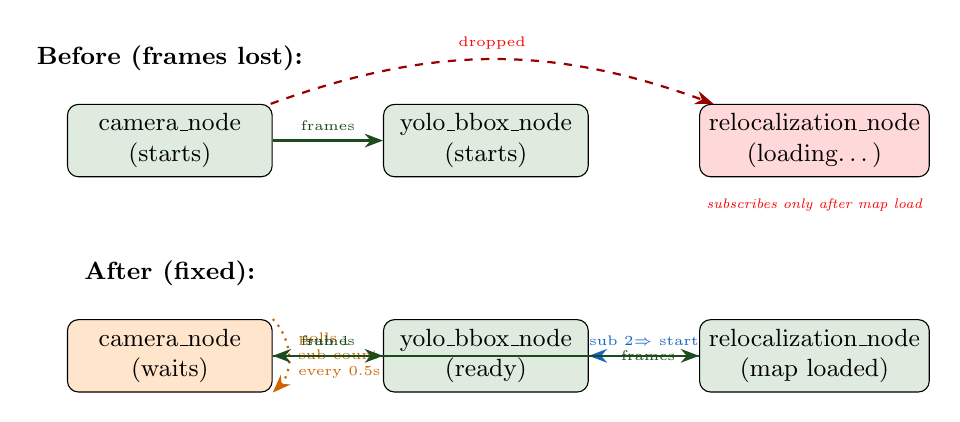
\begin{tikzpicture}[
  node distance=0.5cm and 1.4cm,
  box/.style={draw, rounded corners, minimum height=0.8cm, minimum width=2.6cm,
              align=center, font=\small},
  arrow/.style={-{Stealth}, thick},
  timeline/.style={draw=gray!50, dashed}
]

% ── BEFORE ────────────────────────────────────────────────────────────────────
\node[box, fill=green!15] (cam_b)  {camera\_node\\(starts)};
\node[box, fill=green!15, right=of cam_b] (yolo_b) {yolo\_bbox\_node\\(starts)};
\node[box, fill=red!15,   right=of yolo_b] (rel_b)  {relocalization\_node\\(loading\ldots)};

\node[font=\small\bfseries, above=0.3cm of cam_b] (before_label) {Before (frames lost):};

\draw[arrow, color=green!60!black]  (cam_b)  -- node[above,font=\tiny]{frames} (yolo_b);
\draw[arrow, color=red!60!black, dashed]    (cam_b)  to[bend left=20]
    node[above,font=\tiny,color=red]{dropped} (rel_b);

\node[below=0.15cm of rel_b, font=\tiny\itshape, color=red]
    {subscribes only after map load};

% ── AFTER ─────────────────────────────────────────────────────────────────────
\node[box, fill=orange!20, below=1.8cm of cam_b] (cam_a)
    {camera\_node\\(waits)};
\node[box, fill=green!15, right=of cam_a] (yolo_a) {yolo\_bbox\_node\\(ready)};
\node[box, fill=green!15, right=of yolo_a] (rel_a)
    {relocalization\_node\\(map loaded)};

\node[font=\small\bfseries, above=0.3cm of cam_a] (after_label) {After (fixed):};

% poll arrow
\draw[arrow, dotted, color=orange!80!black] (cam_a.north east)
    to[bend left=45]
    node[right, font=\tiny, align=left]{polls\\sub count\\every 0.5s}
    (cam_a.south east);

\draw[arrow, color=green!60!black] (yolo_a) -- node[above,font=\tiny]{sub 1} (cam_a);
\draw[arrow, color=primary]        (rel_a)  -- node[above,font=\tiny]{sub 2\\$\Rightarrow$ start} (yolo_a);

\draw[arrow, color=green!60!black] (cam_a) -- node[above,font=\tiny]{frames} (yolo_a);
\draw[arrow, color=green!60!black] (cam_a) -- ++(5.6,0)
    node[right,font=\tiny]{frames} |- (rel_a);

\end{tikzpicture}
\caption{Startup sequence before and after the race-condition fix.}
\end{figure}

\subsection{Camera node: subscriber polling}

The camera node now starts a 0.5\,Hz polling timer in place of the immediate
publish timer. Publishing begins only when at least two subscribers are
detected on \texttt{/camera/image\_raw} --- one from the YOLO node and one
from the relocalization node.

\begin{lstlisting}[style=python, caption={\texttt{camera\_node.py} --- subscriber wait logic}]
# In __init__: replaced create_timer(fps, publish_frame)
self.get_logger().info('Waiting for subscribers on /camera/image_raw ...')
self._pub_timer  = None
self._wait_timer = self.create_timer(0.5, self._wait_for_subscribers)

def _wait_for_subscribers(self):
    if self.pub.get_subscription_count() >= 2:
        self._wait_timer.cancel()
        self.get_logger().info(
            f'{self.pub.get_subscription_count()} subscriber(s) connected'
            ' — starting frame publishing')
        self._pub_timer = self.create_timer(1.0 / self._fps, self.publish_frame)
\end{lstlisting}

\subsection{Relocalization node: late subscription}

The root fix is in the relocalization node constructor. Previously, both topic
subscriptions were created \emph{before} \texttt{loadMap()} was called, so the
node registered as a subscriber while the map was still loading. The
subscriptions were moved to \emph{after} \texttt{ready\_ = true}:

\begin{lstlisting}[style=cpp, caption={Subscription creation moved to after map load (\texttt{relocalization\_node.cpp})}]
// ...load vocab, load map, open CSV log...
ready_ = true;

// Subscribe only after map is loaded so camera_node doesn't start
// publishing until this node is truly ready to process frames.
image_sub_ = create_subscription<sensor_msgs::msg::Image>(
    "/camera/image_raw", 10, ...);
yolo_sub_  = create_subscription<std_msgs::msg::String>(
    "yolo/results", 10, ...);
\end{lstlisting}

The guaranteed startup sequence is now: camera waits $\to$ YOLO subscribes (count~=~1) $\to$ relocalization finishes loading and subscribes (count~=~2) $\to$ camera starts publishing.

% ─────────────────────────────────────────────────────────────────────────────
\section{Navigation Stack}

Commit \texttt{fda19a6} added a complete navigation package (\texttt{src/navigation/}) on top of the existing A* skeleton. The package now has four entry points that are co-launched by \texttt{nav.launch.py}.

\subsection{Architecture}

\begin{figure}[H]
\centering
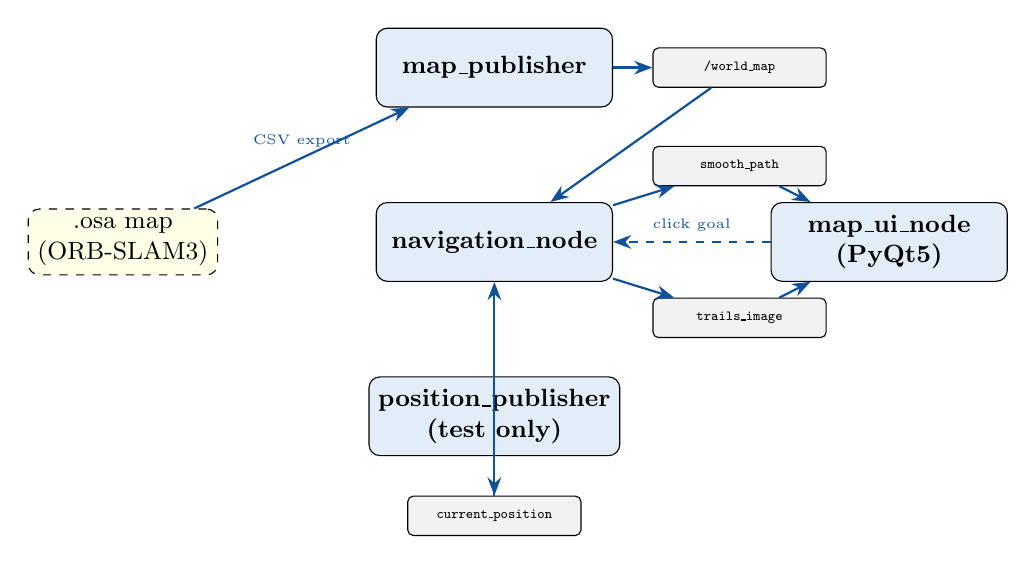
\begin{tikzpicture}[
  node distance=0.6cm and 1.5cm,
  rosnode/.style={draw, rounded corners, fill=primary!12, minimum height=1.0cm,
                  minimum width=3.0cm, align=center, font=\small\bfseries},
  topic/.style={draw, fill=gray!10, minimum height=0.5cm,
                minimum width=2.2cm, align=center, font=\tiny, rounded corners=2pt},
  arrow/.style={-{Stealth}, thick, color=primary!80!black},
  ext/.style={draw, dashed, fill=yellow!10, rounded corners,
              minimum height=0.8cm, minimum width=2.4cm, align=center, font=\small}
]

\node[rosnode] (mp)  {map\_publisher};
\node[rosnode, below=1.2cm of mp]  (nn)  {navigation\_node};
\node[rosnode, right=2cm of nn]    (ui)  {map\_ui\_node\\(PyQt5)};
\node[rosnode, below=1.2cm of nn]  (pp)  {position\_publisher\\(test only)};
\node[ext,     left=2cm of nn]     (osa) {.osa map\\(ORB-SLAM3)};

\node[topic, right=0.5cm of mp] (wm)  {\texttt{/world\_map}};
\node[topic, above right=0.2cm and 0.5cm of nn] (sp) {\texttt{smooth\_path}};
\node[topic, below right=0.2cm and 0.5cm of nn] (ti) {\texttt{trails\_image}};
\node[topic, below=0.5cm of pp] (cp)  {\texttt{current\_position}};

\draw[arrow] (osa) -- node[above,font=\tiny]{CSV export} (mp);
\draw[arrow] (mp)  -- (wm);
\draw[arrow] (wm)  -- (nn);
\draw[arrow] (pp)  -- (cp);
\draw[arrow] (cp)  -- (nn);
\draw[arrow] (nn)  -- (sp);
\draw[arrow] (nn)  -- (ti);
\draw[arrow] (sp)  -- (ui);
\draw[arrow] (ti)  -- (ui);
\draw[arrow, dashed] (ui) -- node[above,font=\tiny]{click goal} (nn);

\end{tikzpicture}
\caption{Navigation package node graph.}
\end{figure}

\subsection{Map publisher}

\texttt{map\_publisher.py} converts the exported point-cloud CSV (from the
\texttt{osa\_to\_csv} tool) into a \texttt{nav\_msgs/OccupancyGrid} and
publishes it at 1\,Hz on \texttt{/world\_map}. It also saves a PNG image of
the occupancy map so the UI can offer a map-selection dropdown. The grid
resolution and dilation radius are configurable parameters.

\subsection{A* path planner}

\texttt{NavigationNode} subscribes to the occupancy grid, the robot's current
position, and a goal position. It runs \texttt{AStarImplementation} on every
state change and publishes a smoothed path. If the robot deviates more than
25\,pixels from the planned path, replanning is triggered automatically. The
A* heuristic is the Euclidean distance to goal:
\[
  h(n) = \left\|\mathbf{p}_n - \mathbf{p}_{\text{goal}}\right\|_2.
\]
The \texttt{snap\_to\_free} function corrects goals that fall inside occupied
cells by searching the nearest free cell in a spiral pattern.

\subsection{PyQt5 UI}

\texttt{map\_ui\_node.py} provides a graphical interface where the user can
select a map PNG from a dropdown (auto-refreshed when new PNGs are detected),
click on the map to set a navigation goal, and observe the live trail image
published by the planner.

\subsection{Tools: \texttt{osa\_to\_csv} and \texttt{map\_to\_csv}}

Two C++ tools were added to extract map data from ORB-SLAM3 atlas files
(\texttt{.osa}) into CSV point clouds, which the map publisher then consumes.
These tools link against the ORB-SLAM3 library and use a Pangolin stub header
to avoid requiring a display during export.

% ─────────────────────────────────────────────────────────────────────────────
\section{Summary}

The five commits since \texttt{32a4119} significantly expanded the system in
two directions. On the evaluation side, the ground-truth comparison pipeline
now produces meaningful accuracy numbers: after Umeyama alignment the
relocalization error is approximately 5\,cm mean APE, which is well within
acceptable range for indoor navigation. On the execution side, a long-standing
startup race condition was eliminated so that every frame processed by the
YOLO and relocalization nodes is guaranteed to originate from after both
subscribers are fully initialised. The navigation stack adds end-to-end path
planning from an ORB-SLAM3 map through A* to a visual PyQt5 interface,
completing the pipeline from map creation to robot guidance.

\vspace{1em}
\begin{tcolorbox}[colback=green!6, colframe=green!60!black,
  fonttitle=\bfseries, title={Tuning Reference}]
\textbf{Landmark vs.\ background weight:} edit \texttt{landmark\_weight} and
\texttt{background\_weight} constants near line 228 of
\texttt{relocalization\_node.cpp}.\\[4pt]
\textbf{Per-class weight:} add \texttt{case} entries to
\texttt{getSemanticWeight()} in \texttt{relocalization.cpp}.\\[4pt]
\textbf{Alignment:} Umeyama has no parameters; it is a closed-form SVD
solution fitted to all matched frames.
\end{tcolorbox}

\end{document}
